\subsection{Ethylene oxidation in a partially-stirred reactor}

\citet{manzello2007soot} utilized a well-stirred reactor (WSR) connected to a flow reactor to study soot formation during ethylene oxidation at equivalence ratios, $\phi=$ 1.9, 2.0, and 2.1, and provided PSD measurements at the end of flow reactor using nano-differential mobility analyzer (Nano-DMA). The WSR had the same size of the reactor used by \citet{manzello2007soot} and explained in Sec.\ref{sec:psrvalid}. The flow reactor is 70 cm long with an inner diameter of 5.1 cm. A coupled PSR-PFR reactor model of omnisoot was used to simulate soot formation during the combustion and flow evolution in the device. The nominal residence time, $\tau$ of flow in the PSR is 11 ms~\citep{manzello2007soot}. The reactants are assumed to enter PSR at 300 K with an inlet mass flow rate, $\dot{m}_{in}=\rho V / \tau$ where $\rho$ was calculated at reactor temperature of 1723 K suggested by~\citet{lenhert2009effects}. The PFR is assumed to be adiabatic. The calculated average axial velocity in the PFR is 14.5 m/s close to the values suggested by~\citet{manzello2007soot}. KAUST mechanism was used to describe gas chemistry. 

The inception and PAH adsorption adjustment factors were varied for each PAH growth model to match the predicted PSD with the measurements as closely as possible for all three $\phi$s. As shown in Figure~\ref{fig:psrpfr_psd}, all inception models capture the peak number concentration and the unimodal shape of the PSD, which indicates that particle inception has ceased, and coagulation is the dominant mechanism for agglomerate size growth. As reported in Table~\ref{tab:psrpfr_morpcomp}, the geometric mean mobility diameter, $d_{m,g}$ and the geometric mobility standard deviation, $\sigma_{m,g}$ obtained using all inception models are in good agreement with the values calculated from the measured PSD~\citep{manzello2007soot}. As it can be seen in Figure~\ref{fig:psrpfr_psd}-(a) \& (b), the spread of predicted PSD is narrower than that of measurements for $\phi$=1.9 and 2.1, which corresponds to under-prediction of $\sigma_{m,g}$ for these equivalence ratios.


\begin{figure}[H]
	\centering
	\begin{tikzpicture}
		\draw (0, 0) node[inner sep=0] 	{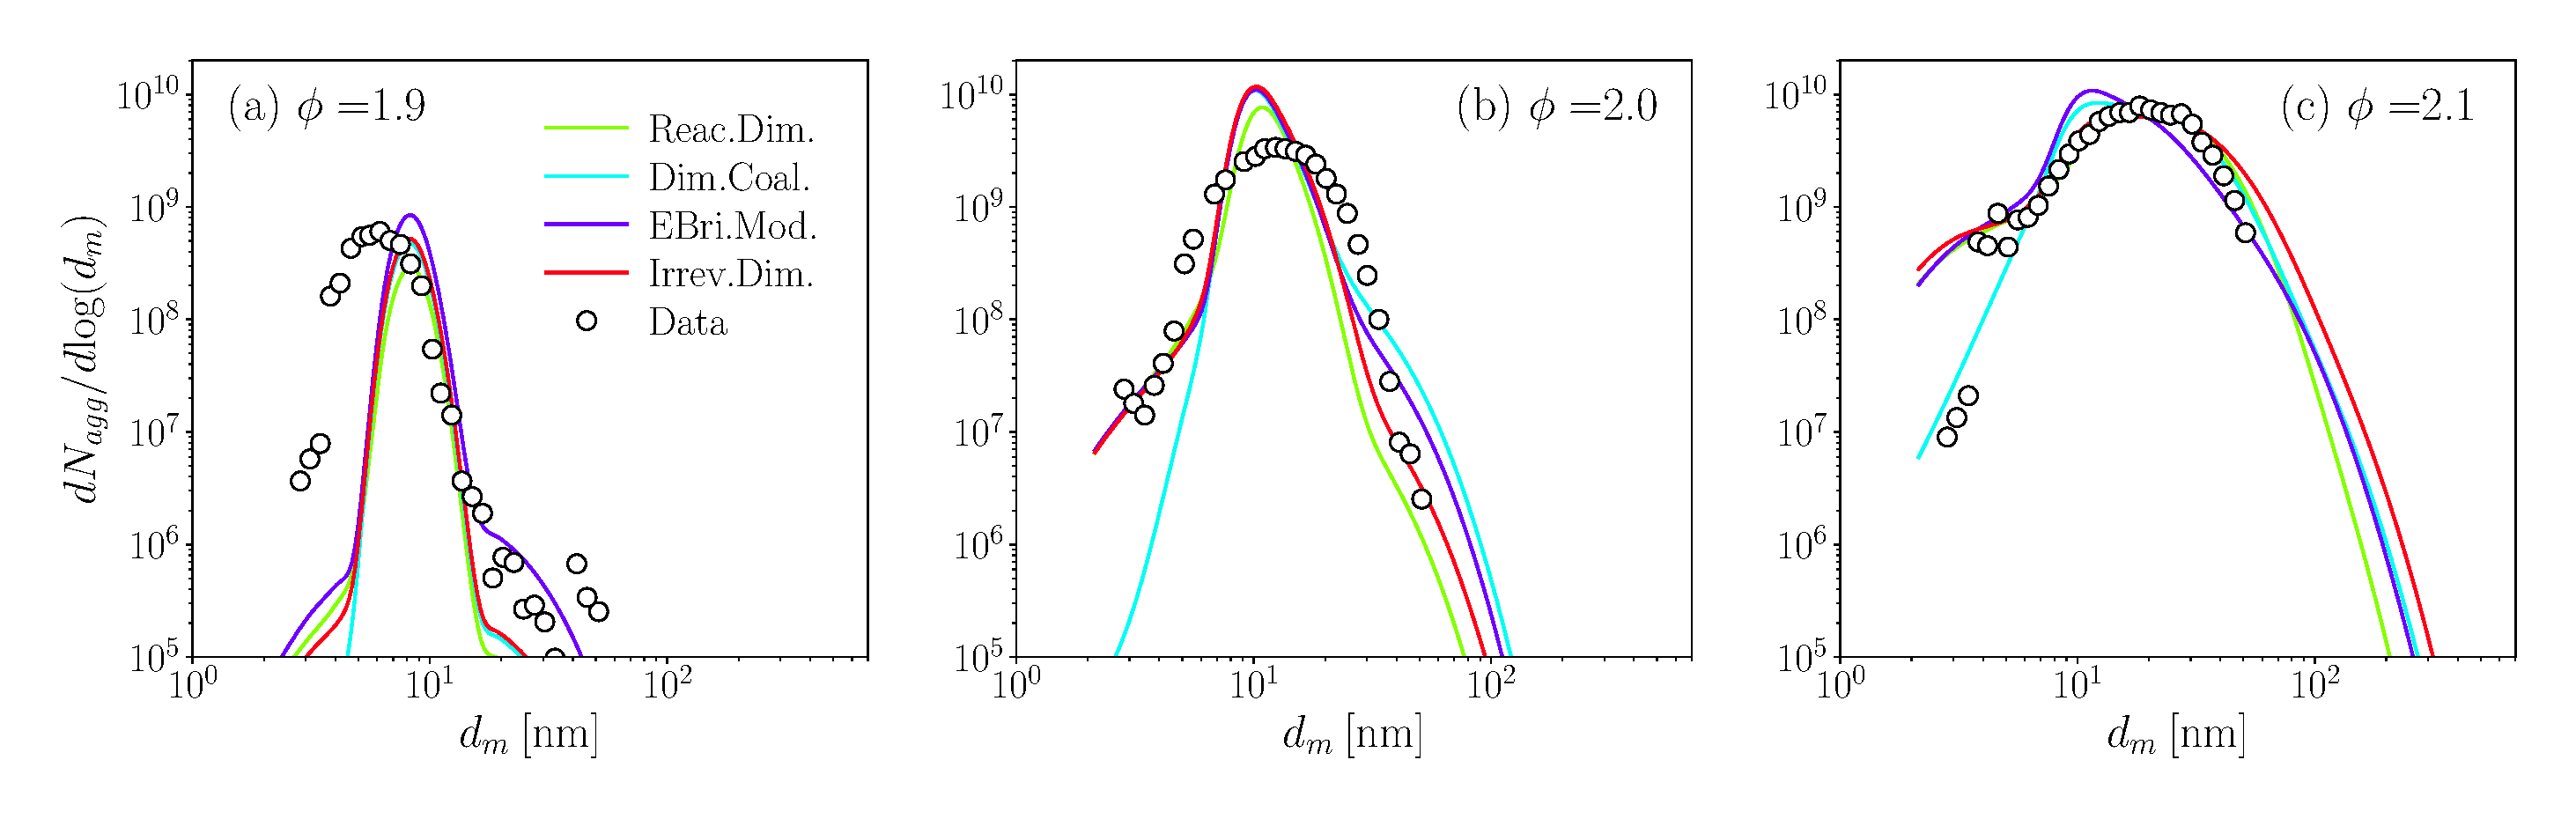
\includegraphics[width=1\textwidth]{Figures/Results/PSR/PSD_eq_ratio_log.pdf}};
		\draw (-3.05, 0.55) node {\tiny{\cite{manzello2007soot}}};
		%\draw (1.95, 0.66) node {\tiny{\cite{manzello2007soot}}};
		%\draw (5.5, -1.28) node {\tiny{\cite{manzello2007soot}}};
	\end{tikzpicture}
	\caption{The particle size distribution at the end of PFR for $\phi$=1.9 (a), 2.0 (b), and 2.1 (c) obtained using KAUST mechanism and different inception models calibrated to match the predictions with measurement~\citep{manzello2007soot}.}
	\label{fig:psrpfr_psd} 
\end{figure}


\begin{table}[H]
	\centering
	\caption{The geometric mean mobility diameter, $d_{m,g}$, and the geometric mobility standard deviation, $\sigma_{m,g}$ obtained using different inception models compared with the value calculated from the measured PSD~\citep{manzello2007soot}}
	\label{tab:psrpfr_morpcomp}
	\begin{tabular}{l|ll|ll|ll|}
		\cline{2-7}
		& \multicolumn{2}{c|}{$\phi=$1.9}                   & \multicolumn{2}{c|}{$\phi=$2.0} & \multicolumn{2}{c|}{$\phi=$2.1} \\ \cline{2-7} 
		& \multicolumn{1}{l} {$d_{m,g}$  [nm]} & $\sigma_{m,g}$ & \multicolumn{1}{l} {$d_{m,g}$  [nm]} &  $\sigma_{m,g}$ & \multicolumn{1}{l}{$d_{m,g}$  [nm]} & $\sigma_{m,g}$ \\ \hline
		\multicolumn{1}{|l|}{Data~\citep{manzello2007soot}}                      & \multicolumn{1}{l}{6.04}          &     1.25      & \multicolumn{1}{l}{12.40} &  1.49 & \multicolumn{1}{l}{17.66} & 1.64 \\ \hline
		\multicolumn{1}{|l|}{Reactive Dimerization}     & \multicolumn{1}{l}{8.27}          &    1.14       & \multicolumn{1}{l}{11.10} & 1.21  & \multicolumn{1}{l}{16.88} & 1.58  \\ \hline
		\multicolumn{1}{|l|}{Dimer Coalescence}         & \multicolumn{1}{l}{8.18}          &      1.14     & \multicolumn{1}{l}{10.76} & 1.24 & \multicolumn{1}{l}{16.99} & 1.68 \\ \hline
		\multicolumn{1}{|l|}{EBridge Modified}          & \multicolumn{1}{l}{8.27}          &    1.15       & \multicolumn{1}{l}{11.02} & 1.27 & \multicolumn{1}{l}{14.56} & 1.58 \\ \hline
		\multicolumn{1}{|l|}{Irreversible Dimerization} & \multicolumn{1}{l}{8.19}          &      1.14     & \multicolumn{1}{l}{10.96} & 1.25 & \multicolumn{1}{l}{18.44} & 1.78 \\ \hline
	\end{tabular}
\end{table}

All inception models underpredict the number concentration of small particles ($d_m<$6 nm) at $\phi$=1.9. The discrepancy decreases for $\phi$=2 and the model predictions align well with the measurements. The number concentration of the smallest measured particle ($\approx$2 nm) is less affected by equivalence ratio compared to the numerical results. This suggests a stronger sensitivity of the PAH production rate to variation of $\phi$ from 1.9 to 2.1, which directly impacts soot inception flux. The strong similarity of profiles of acenaphthylene (A2R5) mole fraction and soot inception along the reactor shown in Fig~.\ref{fig:psrpfr_Iinc_PAH} highlights the dominant role of PAH chemistry on soot inception. Another important observation is that A2R5 mole fraction is not affected by the employed inception model. One order of magnitude increase in peak A2R5 mole fraction due to the change of $\phi$ from 1.9 to 2.1 is amplified leading to two orders of magnitude increase in inception flux. 

As shown in Figure~\ref{fig:psrpfr_dp}, primary particle diameter, $d_p$ along the flow reactor is nearly the same for all inception models at $\phi$=1.9, but the difference becomes noticeable for higher $\phi$ values. Reactive Dimerization predicts the largest final $d_p$ because it directs more PAH mass to surface growth rather than inception, which is consistent with lower peak number concentration observed in Figure~\ref{fig:psrpfr_psd}. $d_p$ rapidly decreases at the beginning of the reactor flow due to the rise in the production of incipient particles (spherical particles with diameter of 2 nm ) that lowers the mean $d_p$ of particles. Then, $d_p$ increases by surface growth towards the end of reactor. The final $d_p$ slightly increases with $\phi$, but its range is similar for $\phi$ values. As shown in Figure~\ref{fig:psrpfr_fv}, soot volume fraction however is very sensitive to equivalence ratio, which can be explained by the strong effect of equivalence ratio on PAH production, inception flux, and number of particles. The analysis of surface growth rates at end of PFR revealed that more than 95\% of soot mass is gained through HACA. Figure~\ref{fig:psrpfr_Nagg_HACA} illustrates the coupling between number concentration of agglomerates, $N_{agg}$ and HACA growth rate and their change due to equivalence ratio.  


\begin{figure}[H]
	\centering
	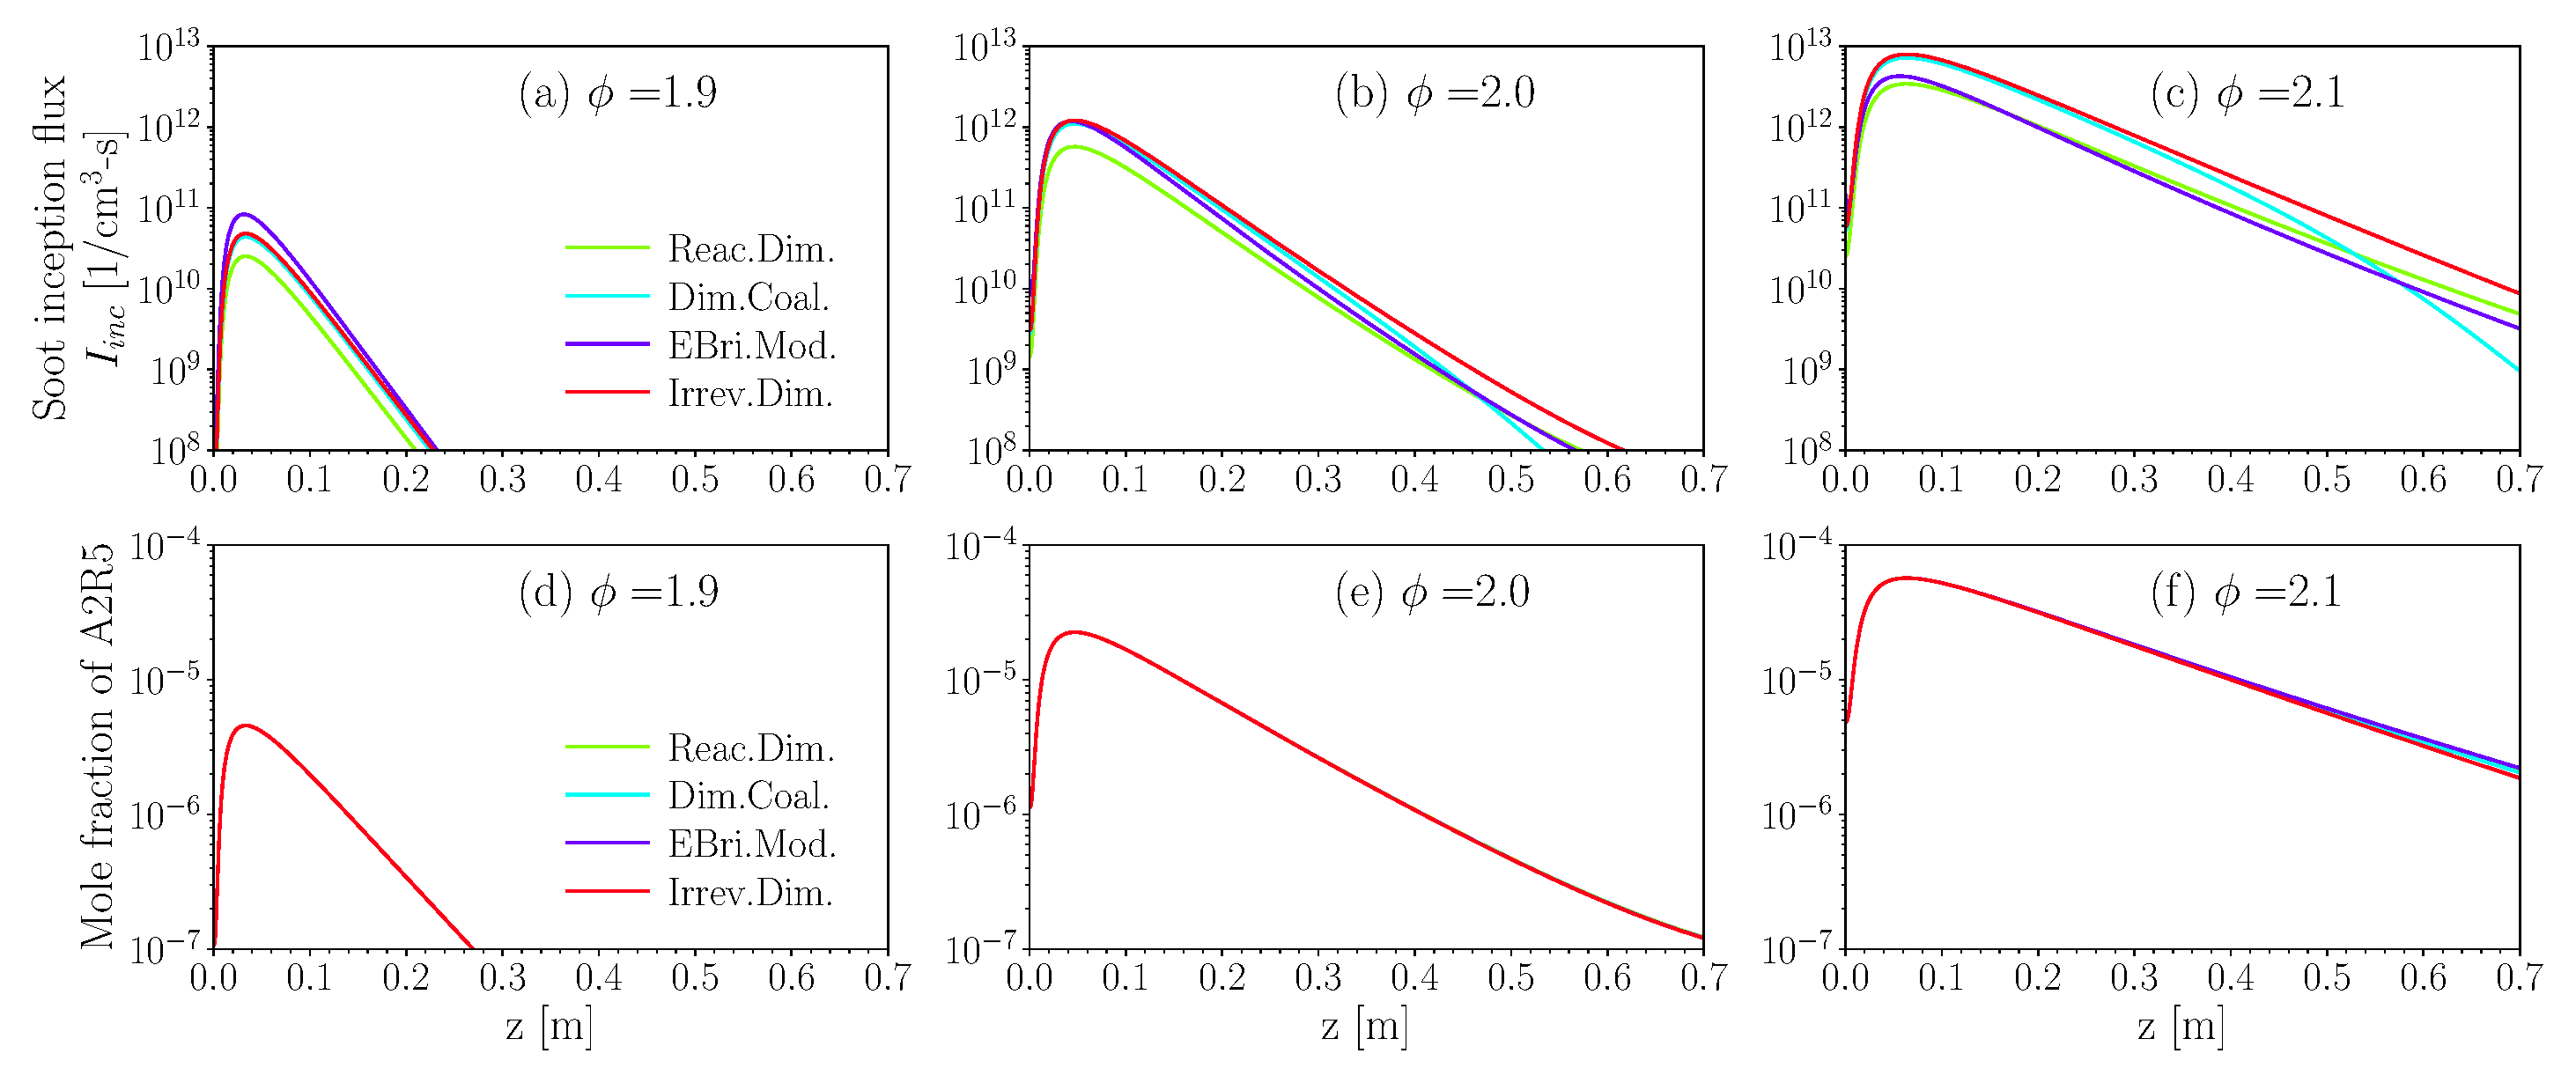
\includegraphics[width=1\textwidth]{Figures/Results/PSR/I_inc_PAH_eq_ratio_all_single_mech.pdf}
	\caption{The soot inception flux, $I_{inc}$ and acenaphthylene, A2R5 mole fraction along the PFR for $\phi$=1.9 (a,d), 2.0 (b,e), and 2.1 (c,f) obtained using KAUST mechanism and different inception models calibrated to match the predictions with measurement~\citep{manzello2007soot}.}
	\label{fig:psrpfr_Iinc_PAH} 
\end{figure}

\begin{figure}[H]
	\centering
	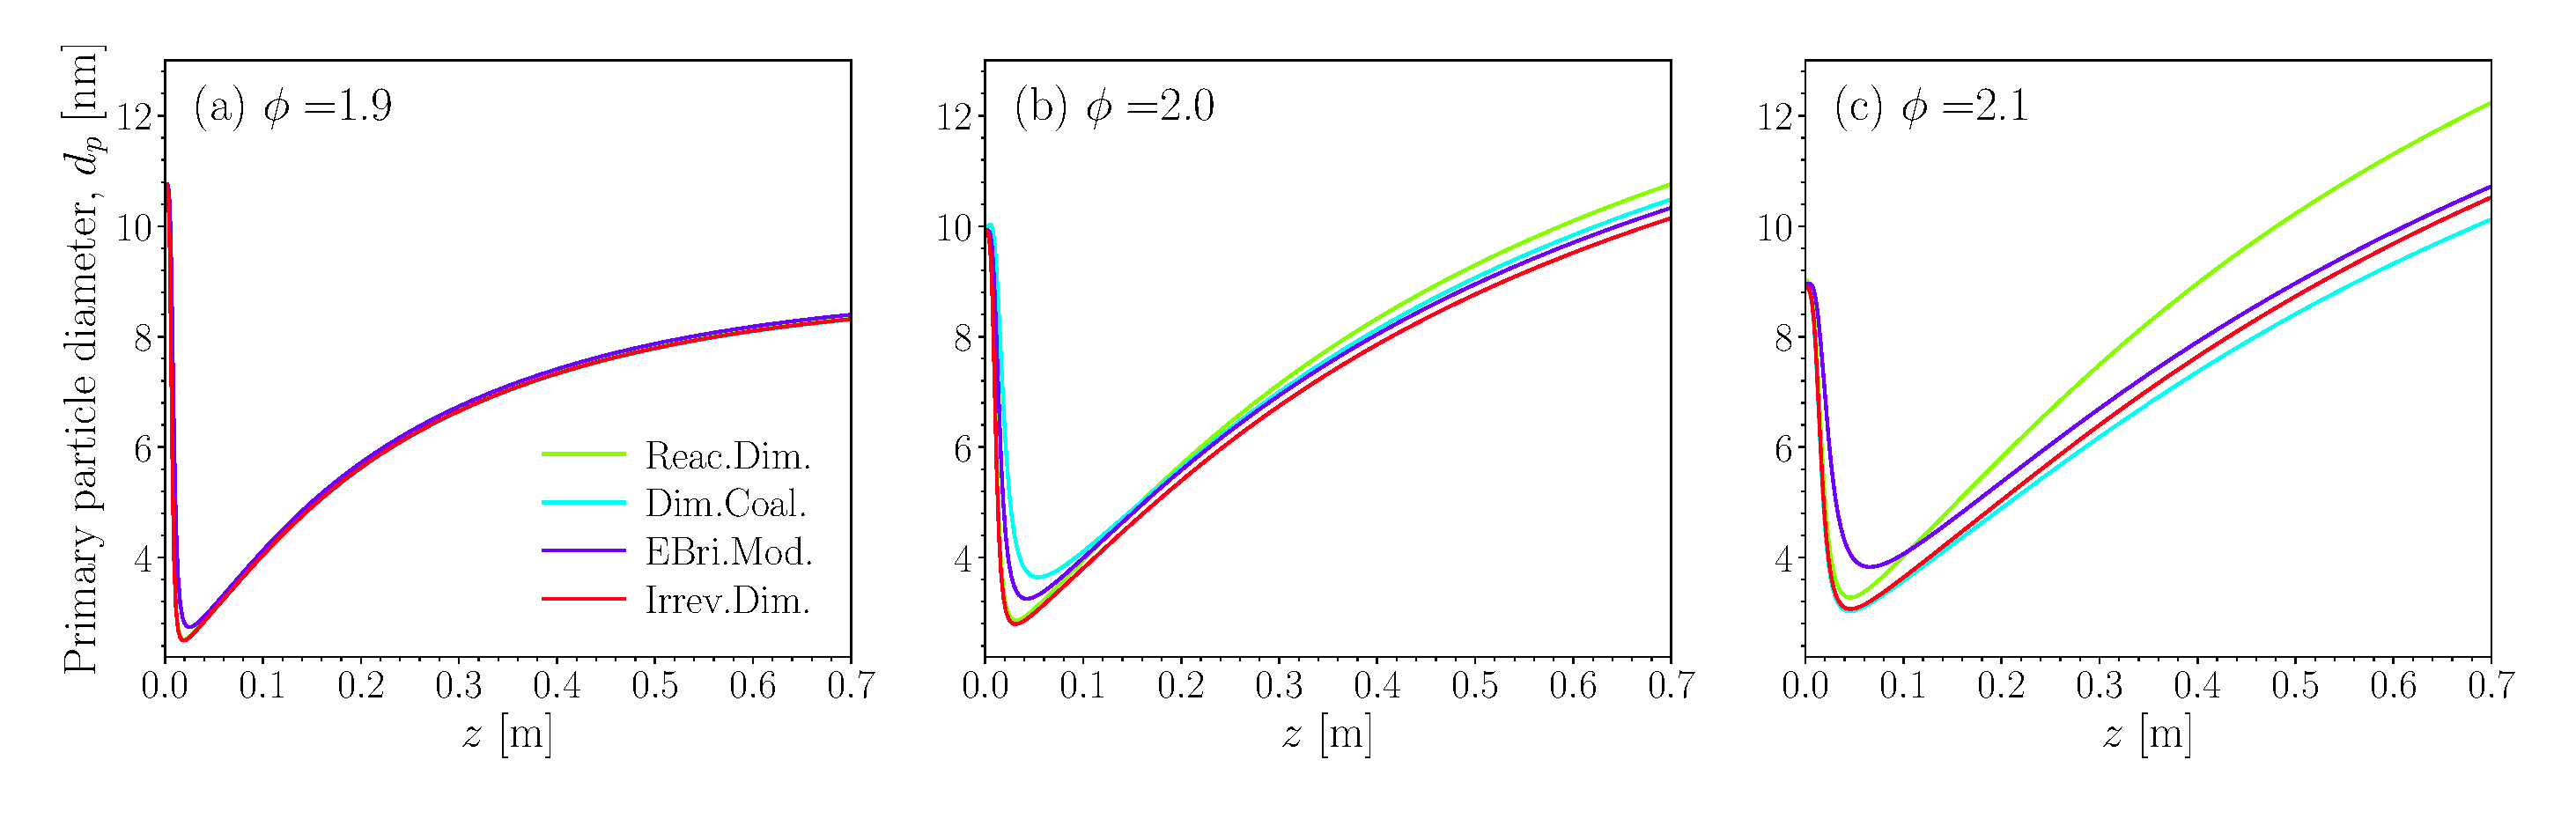
\includegraphics[width=1\textwidth]{Figures/Results/PSR/d_p_eq_ratio_all_single_mech.pdf}
	\caption{The primary particle diameter, $d_p$ along the PFR for $\phi$=1.9 (a), 2.0 (b), and 2.1 (c) obtained using KAUST mechanism and different inception models calibrated to match the predictions with measurement~\citep{manzello2007soot}.}
	\label{fig:psrpfr_dp} 
\end{figure}

\begin{figure}[H]
	\centering
	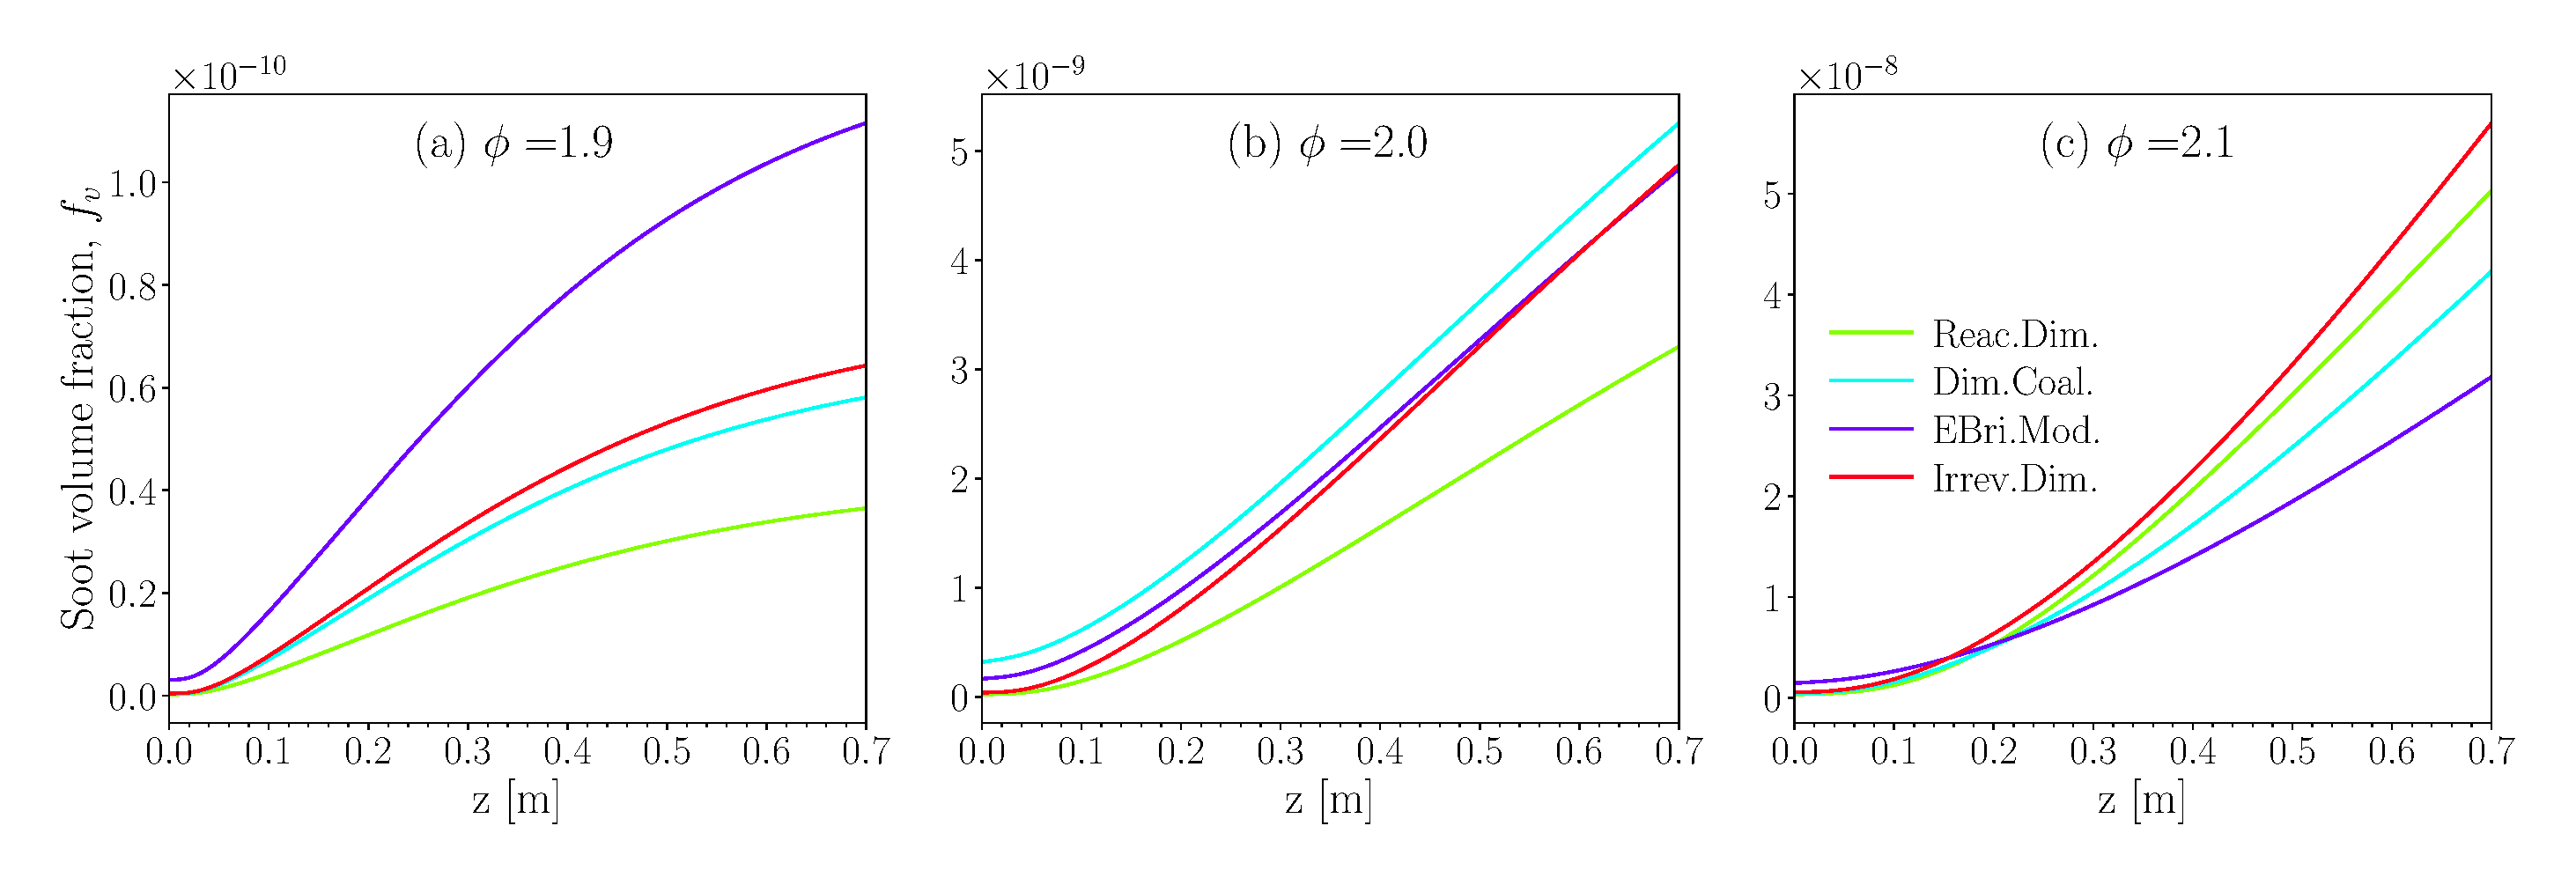
\includegraphics[width=1\textwidth]{Figures/Results/PSR/f_v_eq_ratio_all_single_mech.pdf}
	\caption{The soot volume fraction along the PFR for $\phi$=1.9 (a), 2.0 (b), and 2.1 (c) obtained using KAUST mechanism and different inception models calibrated to match the predictions with measurement~\citep{manzello2007soot}.}
	\label{fig:psrpfr_fv} 
\end{figure}


\begin{figure}[H]
	\centering
	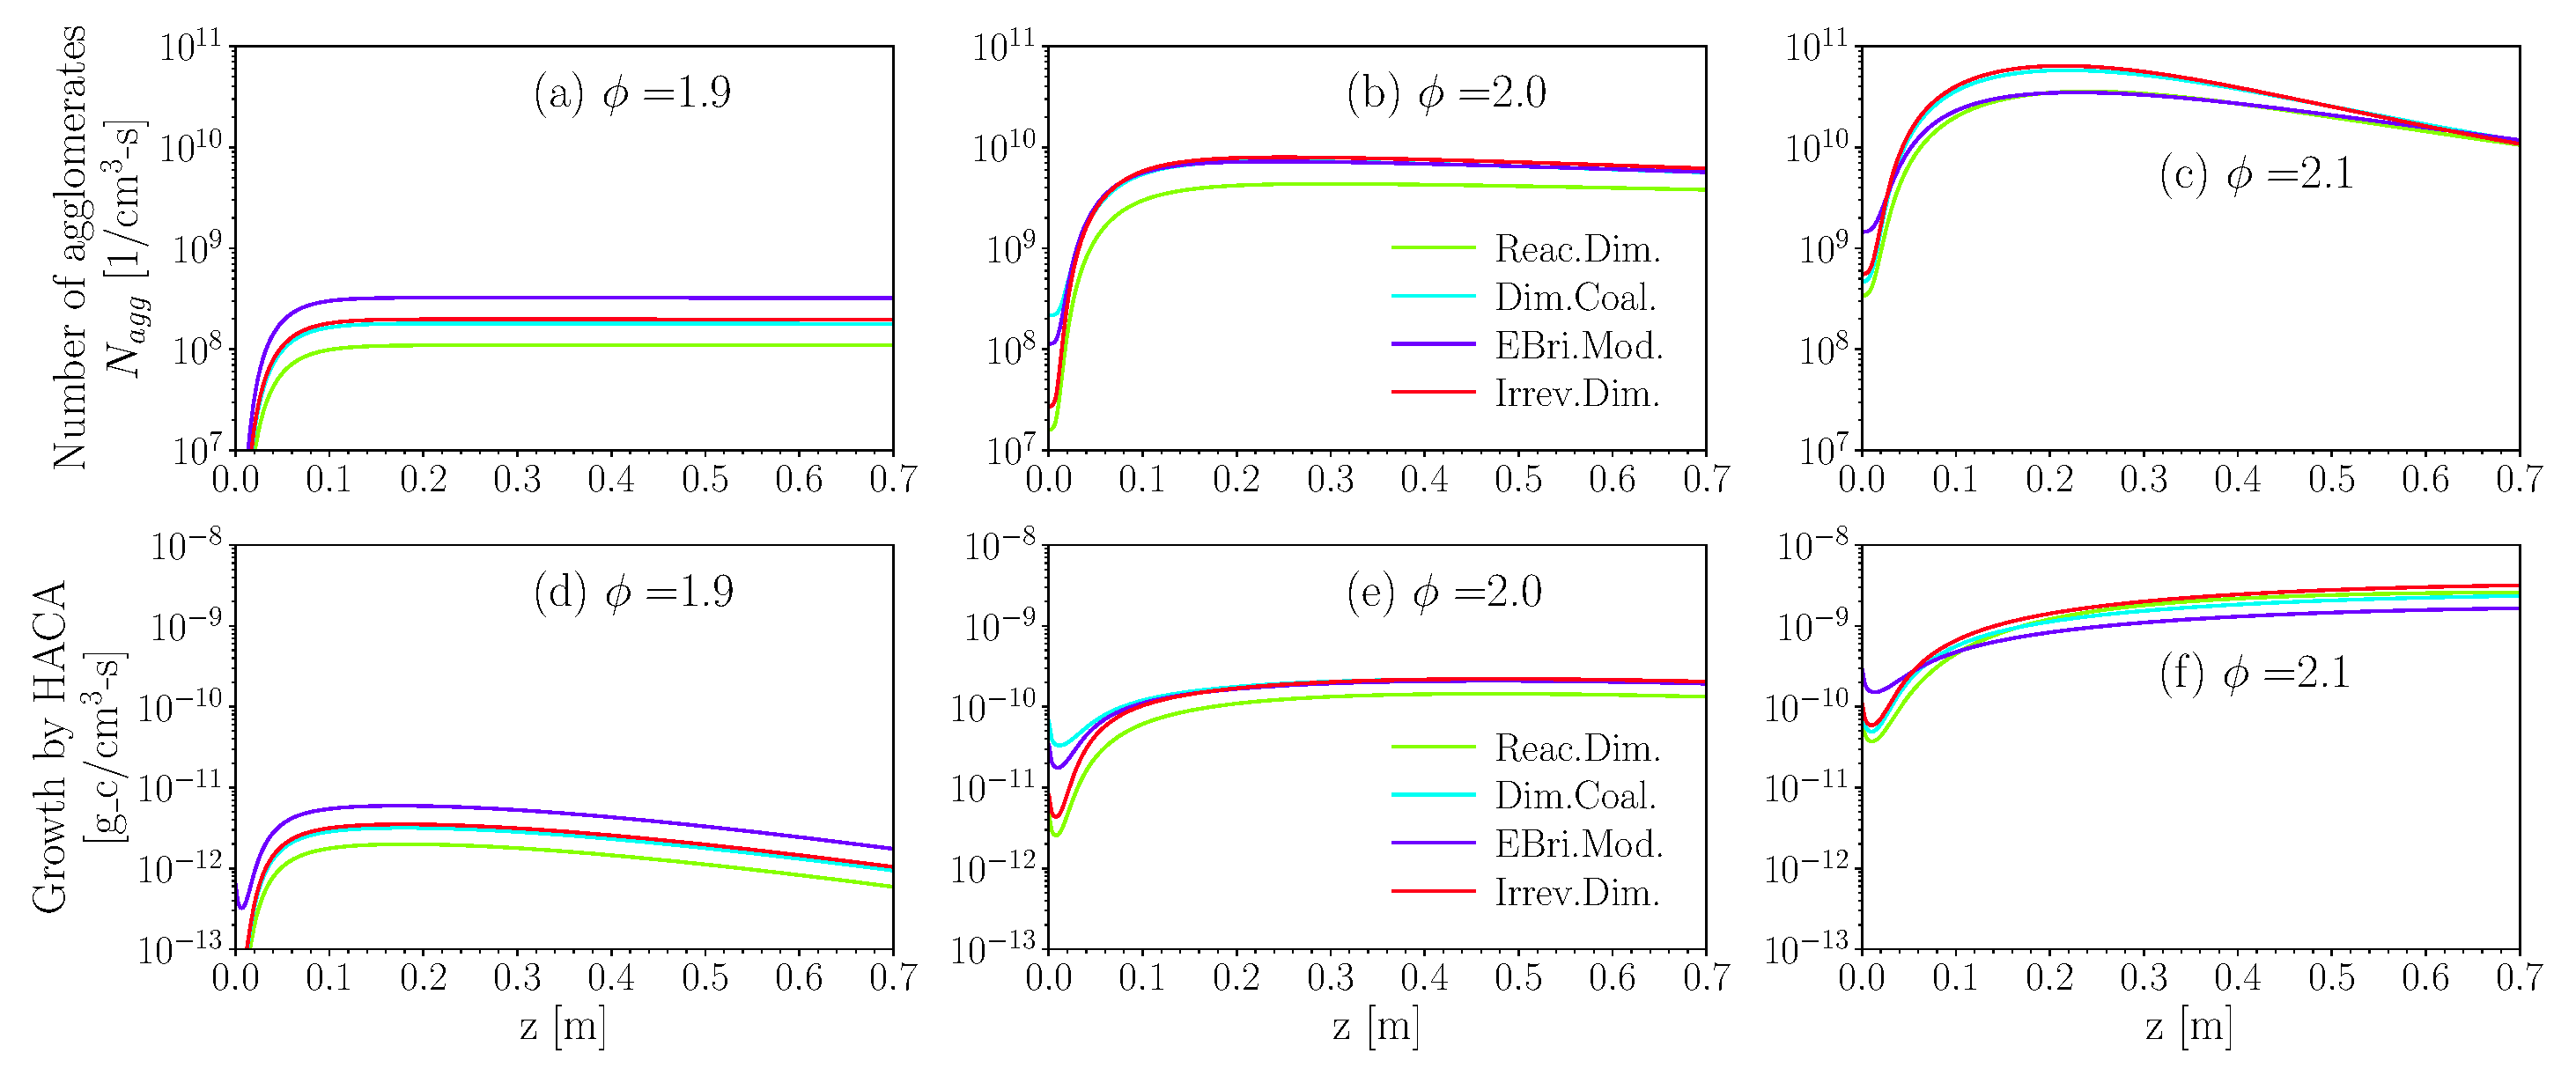
\includegraphics[width=1\textwidth]{Figures/Results/PSR/N_agg_HACA_eq_ratio_all_single_mech.pdf}
	\caption{The number of agglomerates, $N_{agg}$ and the rate of carbon addition by HACA  along the PFR for $\phi$=1.9 (a,d), 2.0 (b,e), and 2.1 (c,f) obtained using KAUST mechanism and different inception models calibrated to match the predictions with measurement~\citep{manzello2007soot}.}
	\label{fig:psrpfr_Nagg_HACA} 
\end{figure}

